\documentclass{article}
\usepackage{xcolor}
\usepackage{titleps}
\usepackage[letterpaper, margin=0.95in]{geometry}
\usepackage{url}
\usepackage{amsmath}
\usepackage{amssymb}
\usepackage{wrapfig}
\usepackage{float}
\usepackage{mathtools}
\usepackage{enumitem}
\usepackage{tabu}
\usepackage{parskip}
\usepackage{natbib}
\usepackage{listings}

\usepackage{hyperref}
\usepackage[color=red]{todonotes}
\usepackage{forest}
\definecolor{light-yellow}{HTML}{FFE5CC}

\newpagestyle{ruled}
{\sethead{CMU 16-831}{Intro to Robot Learning}{Fall 2023}\headrule
  \setfoot{}{}{}}
\pagestyle{ruled}

\renewcommand\makeheadrule{\color{black}\rule[-.75\baselineskip]{\linewidth}{0.4pt}}
\renewcommand*\footnoterule{}

\begin{document}
\lstset{basicstyle = \ttfamily,columns=fullflexible,
backgroundcolor = \color{light-yellow}
}

\begin{centering}
    {\Large Assignment 1: Imitation Learning} \\
    \vspace{.25cm}
    \textbf{Andrew ID:} \texttt{kkabeer} \\
    \textbf{Collaborators:} \texttt{ssaha3, hravisan, asenathi}\\ 
\end{centering}

\vspace{.5cm}

\section{Behavioral Cloning}
\subsection{Part 2}

\begin{center}
  \begin{tabular}{ |c|c|c|c|c|c| } 
   \hline
    & Ant & Humanoid & Walker2d & Hopper & HalfCheetah \\ 
    \hline
   Average Return of Training Data & 4713.65 & 10344.51 & 5566.84 & 3772.67 & 4205.77 \\ 
   Standard Deviation of Training Data & 12.19 & 20.98 & 9.23 & 1.94 & 83.03\\ 
   \hline
  \end{tabular}
\end{center}

\subsection{Part 3}

\begin{center}
  \begin{tabular}{ |c|c|c|c|c|c| } 
   \hline
    & Ant & Humanoid & Walker2d & Hopper & HalfCheetah \\ 
    \hline
   Average Return of Evaluation Data & 1502.93 & 314.30 & 342.79 & 805.38 & 2120.04 \\ 
   Standard Deviation of Evaluation Data & 713.67 & 33.77 & 259.76 & 254.06 & 1193.84 \\
   \% Performance of Expert & 31.88\% & 3.04\% & 6.16\% & 21.35\% & 50.41\% \\
   \hline
  \end{tabular}
\end{center}
I am choosing the Ant environment, which has a performance of 31.88\% of the expert, and the Hopper environment, which has a performance of 21.35\% of the expert

The parameters used for all the environments are the following:

Number of iterations: 1

Evaluation Batch size: 5000

Batch Size: 5000

Network size: 2 hidden layers of size 64 each

\subsection{Part 4}

% Insert the image irl_ass1_1.3.png
\begin{figure}[H]
  \centering
  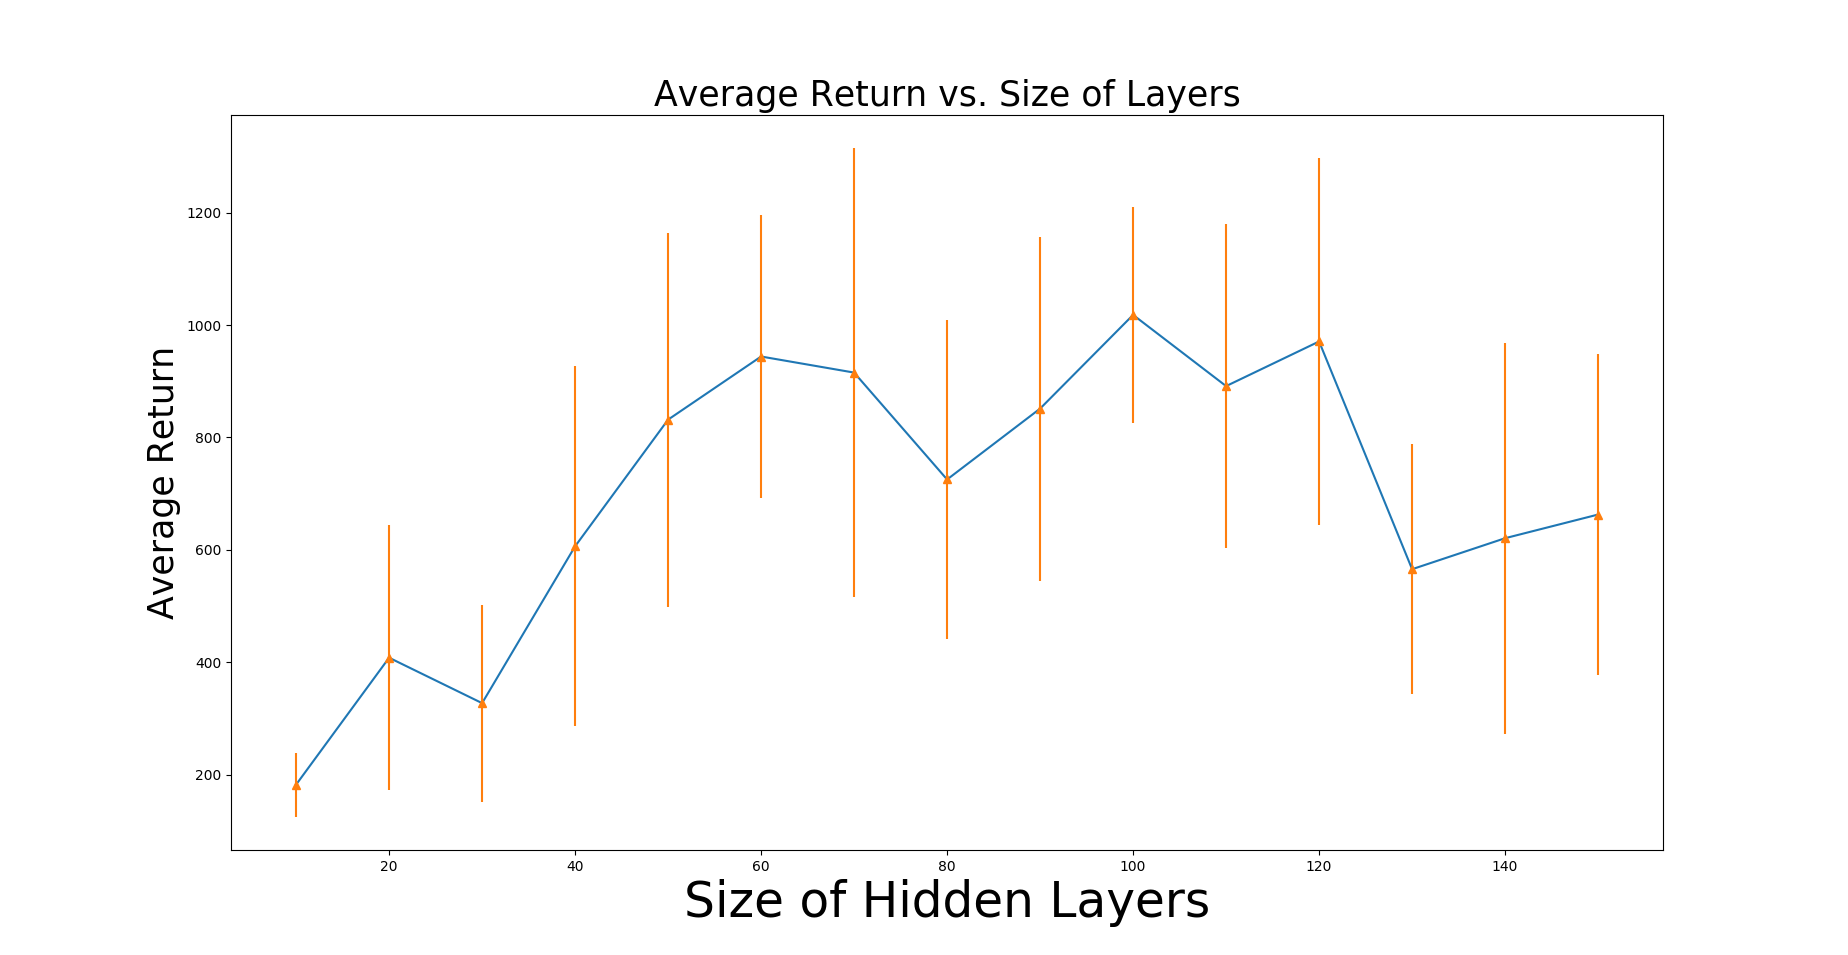
\includegraphics[width=1\linewidth]{irl_ass1_1.3.png}
  \caption{Plot of the average return of the evaluation data vs the size of the hidden layer. I chose this because I felt this parameter would have the most effect on the training of the neural net.}
  \label{fig:1.3}
\end{figure}

The parameters used for the Hopper are the following:

Number of iterations: 1

Evaluation Batch size: 5000

Batch Size: 5000

Network size: 2 hidden layers of variable size (varying from 10 to 150)

\newpage

\section{DAgger}
\subsection{Part 2}

\begin{figure}[H]
  \centering
  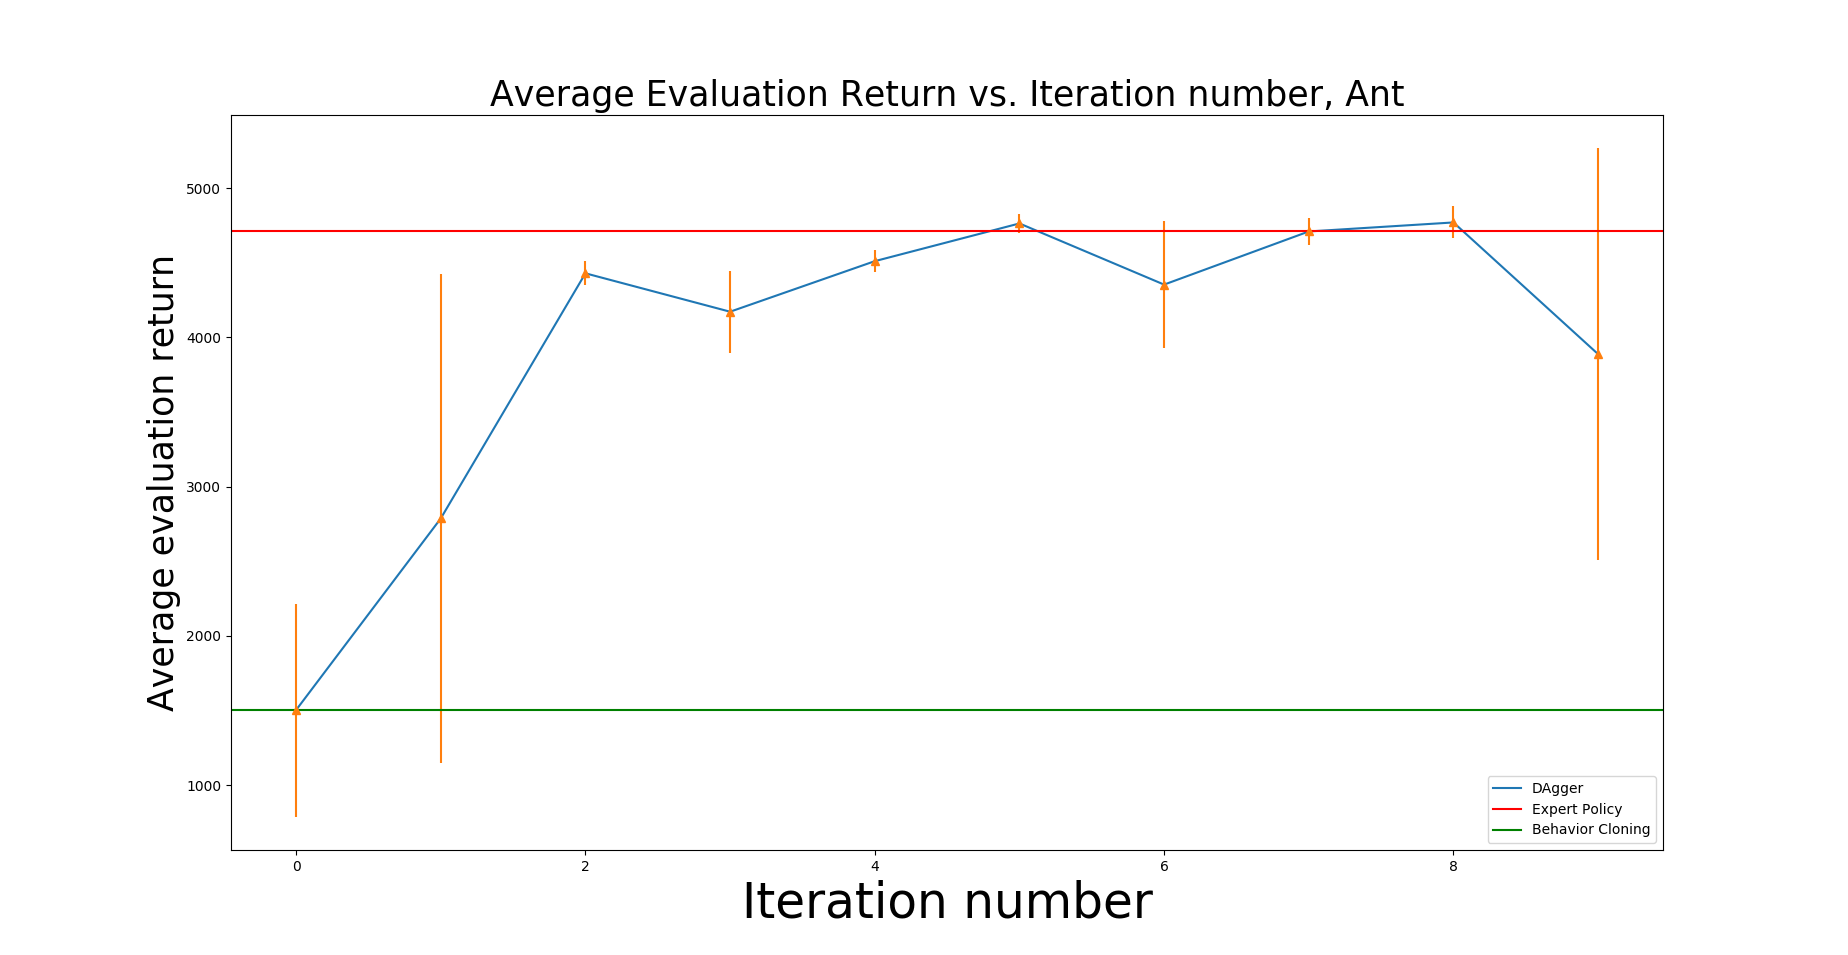
\includegraphics[width=1\linewidth]{irl_ass1_2.1_ant.png}
  \caption{Plot of the average return of the evaluation data vs the iteration number. I chose this because I felt this parameter would have the most effect on the training of the neural net.}
  \label{fig:1.3}
\end{figure}

\begin{figure}[H]
  \centering
  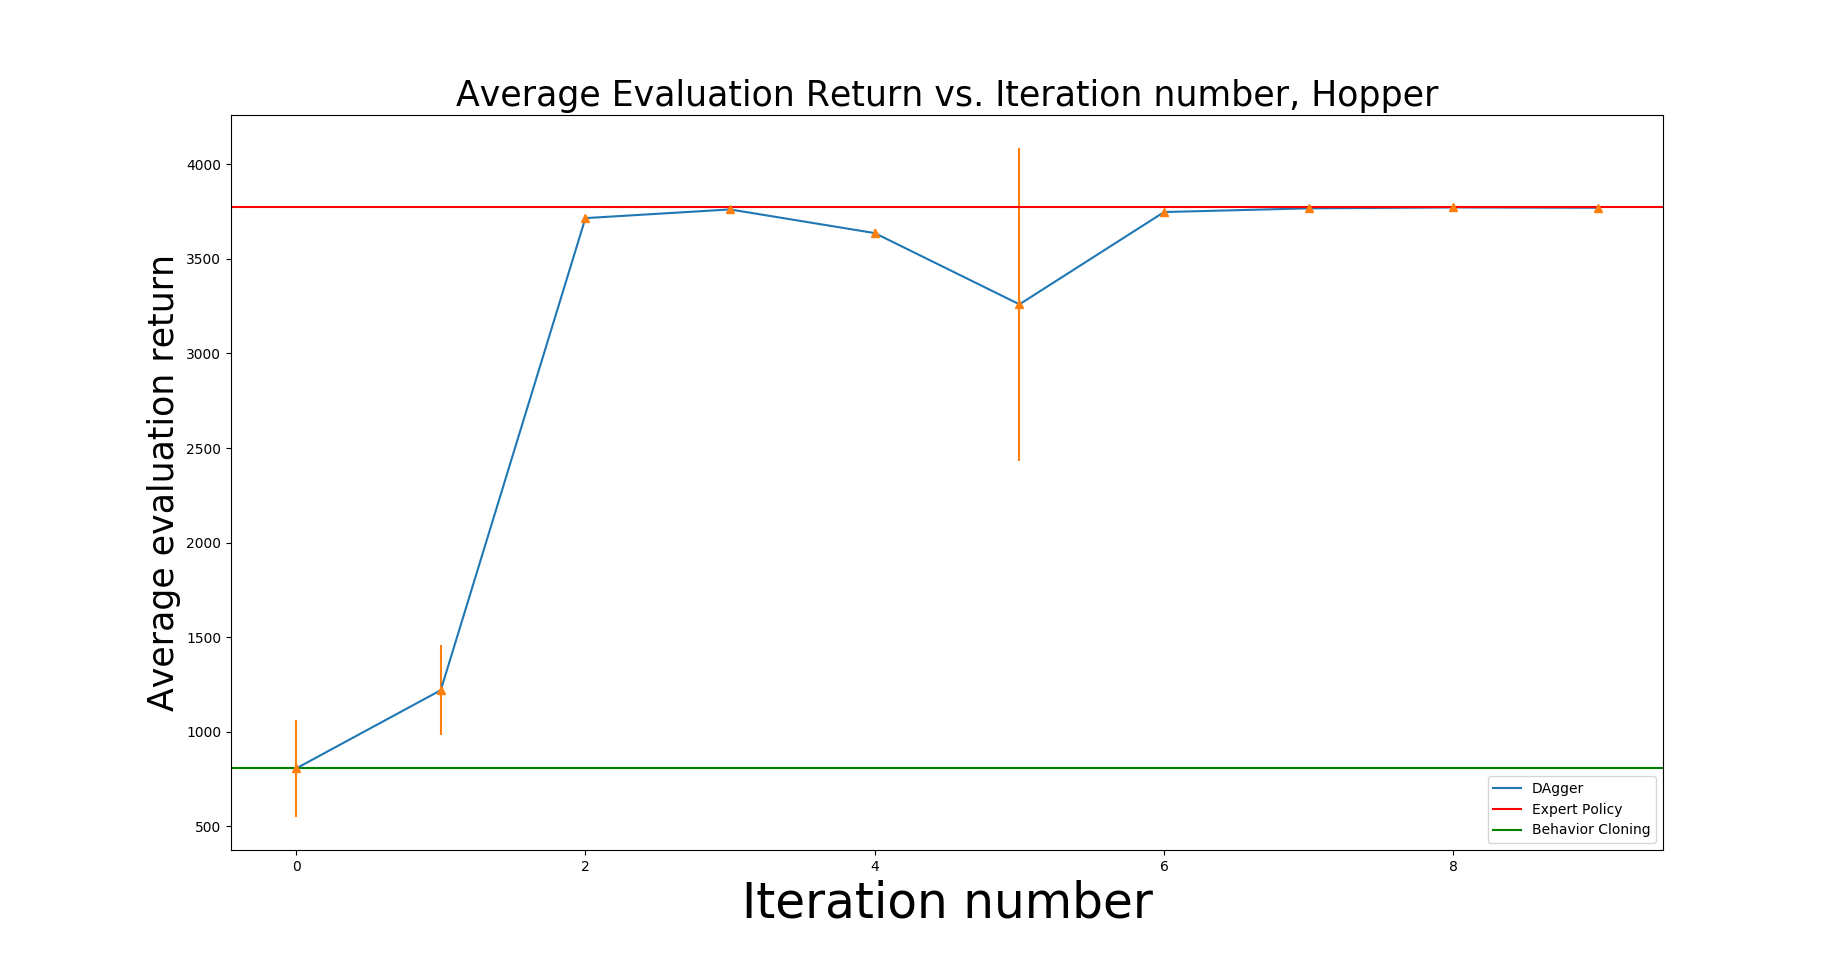
\includegraphics[width=1\linewidth]{irl_ass1_2.1_hopper.png}
  \caption{Plot of the average return of the evaluation data vs the iteration number. I chose this because I felt this parameter would have the most effect on the training of the neural net.}
  \label{fig:1.3}
\end{figure}

The parameters used for both the Hopper and the Ant are the following:

Number of iterations: 10

Evaluation Batch size: 5000

Batch Size: 5000

Network size: 2 hidden layers of size 64 each

\end{document}